\chapter{Data vanuit de Microbit naar SQL sturen}

Dit is het meest complexe deel van de software die je nodig hebt voor ‘The Challenge’. 

Hierin komen 3 vakgebieden samen: Embedded, Java en Databases (SQL).

Bedenk: Dit is slechts een voorbeeld dat laat zien hoe je dat voor de verschillende delen aanpakt.

We gaan er mee om zoals met de eerdere Arduino voorbeelden, zie dit als legoblokjes:

\begin{itemize}
	\item Maak je eigen code erbij voor de Microbit. 
\item In het Java deel voegen jullie een GUI toe.
\item In de database bouwen jullie een structuur met minstens 2 tabellen.
\end{itemize}

Het plaatje hieronder geeft weer wat we gaan doen, zie deze stappen: 

Stap 1: De Microbit meet temperatuur en geeft dit per seconde door via de seriële poort naar de PC. 

Stap 2: Op de PC draait een Java programma die de seriële data vertaalt naar iets bruikbaars.

Stap 3: Het Java programma stopt de data in de SQL database.


\begin{figure}[h!]
	\captionsetup{justification=centering}
	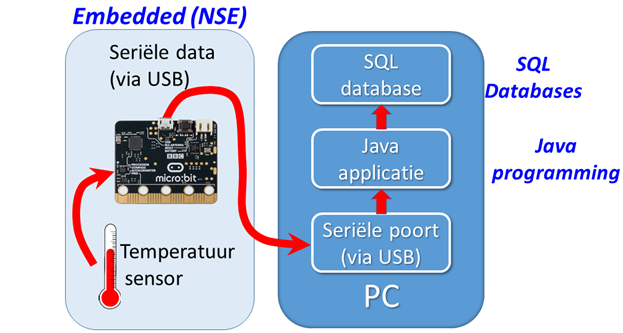
\includegraphics[width=0.6 \linewidth]{figuren/microToSQL}
	\centering
	\caption{Micro:bit naar SQl}
	\label{fig:microSQL}
\end{figure}

Om te zien hoe dit werkt, kijk naar het filmpje \href{https://youtu.be/wZ_bIQh9tME}{"Microbit: Embedded + Java + SQL datalogging"}


\section{Software installeren}

Ik ga er vanuit dat je de volgende software geïnstalleerd hebt:

\begin{itemize}
\item IntelliJ IDE voor Java
\item MySQL database
\end{itemize}

Zo niet, dan staat hieronder waar je het kunt vinden. Zoek zelf uit via de instructies van het vak wat daar precies vereist is.

\paragraph{IntelliJ: }

Deze hebben jullie al geïnstalleerd, daarom geen instructies. Mocht je het nog niet hebben, dit is de link:
\href{https://www.jetbrains.com/idea/download/index.html}{https://www.jetbrains.com/idea/download/index.html}


\paragraph{MySQL:}

Als je Windows gebruikt, download en installeer dan de MySQL Installer (web community versie) vanaf:
\href{https://dev.mysql.com/downloads/installer/}{https://dev.mysql.com/downloads/installer/}


In de installer, selecteer de nieuwste versie van:

\begin{itemize}

\item -MySQL Server
\item -MySQL Workbench

\end{itemize}

(Op 7-12-2019 is dat versie 8.0.18)

\section{Voorbeeld downloaden}


Ga in Blackboard naar de map “Benodigheden voor The Challenge”, “Tips, voorbeeldcode etc.” 

Lees de tekst in de sectie “Informatie, hulpmiddelen en voorbeeldcode”.


Download de voorbeeldcode 
\href{https://blackboard.hhs.nl/bbcswebdav/pid-2889780-dt-content-rid-24452591_2/xid-24452591_2
}{USBserialReceiveToSQL.zip}

Dit bevat het complete project voor het uitlezen van data vanuit de seriële poort en dit in SQL stoppen.

Pak het zip bestand USBserialReceiveToSQL.zip uit naar waar je wilt (map met andere java projecten?)
Je hebt daar nu een map USBserialReceiveToSQL

Start IntelliJ, blader naar bovenstaande map (selecteer de map USBserialReceiveToSQL) en klik OK.

Kies “New window” om het project in een nieuwe instantie van IntelliJ te starten.

\section{Stap 1: Elke seconde een meetwaarde genereren met de Microbit.}

Je kunt op verschillende manieren met de Microbit data genereren om naar de PC te sturen.

Ik heb ervoor gekozen om de temperatuur te meten (elke seconde een meetwaarde; een float). 
Je kunt zelf andere data kiezen, zoals bijvoorbeeld iets van de accelerometer of een code versturen als je een knopje indrukt. \textbf{Je hoeft dus niet elke seconde iets te versturen!} \textit{De Java code wacht eeuwig of er data verzonden wordt vanuit de seriële poort!}

De voorkeursmethode voor programmeren is via Arduino C/C++ code:  

\begin{enumerate}
	\item Open Bestand -> Voorbeelden -> Microbit-HHS -> 07.Temperatuursensor-Bluetooth
	\item Compileer en upload het voorbeeld naar je Microbit.
	\item Open de seriële monitor \colorbox{mygray}{\textbf{(Ctrl+Shift+M)}}, je ziet nu de temperatuurwaardes voorbij komen.
	\item Sluit de seriële monitor weer, anders kan het Java programma er niet bij (er kan maar 1 programma toegang tot de seriële poort hebben).
	
\end{enumerate}


Een alternatieve methode is via Makecode, zie:

 \href{https://makecode.microbit.org/_94Ag85J3s4Yk}{https://makecode.microbit.org/94Ag85J3s4Yk}

Je kunt de uitvoer hiervan ook bekijken met de Arduino seriële monitor. 
Vergeet niet na het kijken de seriële monitor te sluiten!

\section{Stap 2: Data inlezen met Java programma.}

Als het goed is heb je zojuist het voorbeeldprogramma geopend.
Ga in IntelliJ naar ComPortSendReceive.java en comment de volgende regels voor nu even uit 
(met //):

Dit voorkomt dat het programma data schrijft naar de SQL database. Dat kan nog niet, want die heb je nog niet ingericht.

Zorg dat je Microbit aangesloten is en data genereert.

Start in IntelliJ het programma door op het groene driehoekje te klikken (of druk \colorbox{mygray}{\textbf{Shift+F10}}).

Als het goed is zie je in IntelliJ nu de data voorbij komen (datum+tijd en temperatuur).
(met //):


\definecolor{arsenic}{rgb}{0.5, 0.5, 0.5}
\colorbox{arsenic}{
	\begin{minipage}{\textwidth}
		\colorbox{black}{\textcolor{white}{Regel 87:}}:  // InsertIntoSQL \textcolor{purple}{database} = new InsertIntoSQL();\\
	
		\colorbox{black}{\textcolor{white}{Regel 120:}}:  // \textcolor{purple}{database}.insert(tijdstip, temperatuur);
		
	\end{minipage}
}


Dit voorkomt dat het programma data schrijft naar de SQL database. Dat kan nog niet, want die heb je nog niet ingericht.

Zorg dat je Microbit aangesloten is en data genereert.

Start in IntelliJ het programma door op het groene driehoekje te klikken (of druk \colorbox{mygray}{\textbf{Shift+F10}}).

Als het goed is zie je in IntelliJ nu de data voorbij komen (datum+tijd en temperatuur).


\section{Stap 3: Data wegschrijven naar MySQL database.}

Voer de volgende commando's uit in de SQL server om een database, tabel en user aan te maken:

\begin{itemize}
	\item  CREATE DATABASE vb1;
	\item  CREATE TABLE vb1.tbl1(tijdstip TEXT, temperatuur FLOAT);
	\item  CREATE USER microbit IDENTIFIED BY 'geheim';
	\item  GRANT INSERT, UPDATE, SELECT, DELETE ON vb1.* TO 'microbit';
\end{itemize}

Haal de eerder aangebrachte comments in de Java code weg (regels 87 + 120) en start het programma opnieuw. Als het goed is draait het programma nu, zonder foutmeldingen.

Nadat het Java programma data ingevoerd heeft in de database, dan kun je de data opvragen met dit commando:

\begin{itemize}
	\item SELECT * FROM vb1.tbl1;
\end{itemize}

Als je in IntelliJ een foutmelding over de tijd krijgt, dan staat waarschijnlijk in MySQL de tijdzone niet goed. Voer dan dit commando uit op de SQL server:

\begin{itemize}
	\item SET GLOBAL time\_zone = "+1:00"; 
\end{itemize}

\textbf{\textit{Ik ga hier geen uitleg geven over SQL, ik neem aan dat je die in het vak zelf gekregen hebt.
Ook als IntelliJ het niet doet: zoek hulp bij je Java docent!}}

Als je er niet uitkomt, kan deze uitleg van Wouter Pijnacker Hordijk je helpen met foutzoeken en het begrijpen van het programma (totale speelduur ruim een uur):

\href{https://hhs.mediamission.nl/Mediasite/Play/ca2f6403d08e4c86991015797c1c392a1d}{https://hhs.mediamission.nl/Mediasite/Play/ca2f6403d08e4c86991015797c1c392a1d}

Klik op de (i) rechtsonder in het scherm voor een inhoudsopgave en spring naar je onderwerp van keuze.

\section{Stap 4: Eigen aanpassingen maken in Java}

Ga in IntelliJ naar ComPortSendReceive.java en bestudeer de code.\\
Met deze code kun je data verzenden en ontvangen tussen Java en Microbit en SQL.

De door Java ontvangen data wordt verwerkt in onderstaand stuk code. \\
Daar moeten je aanpassingen gebeuren. \\
Bedenk:\textbf{\underline{ Alle data wordt ontvangen en verzonden als tekst! }}
Als je data al tekst is, hoef je dus niks om te zetten! Zie de regel \colorbox{yellow}{String naam = berichtData;}

%\ctext[RGB]{232,209,82}

Hieronder zie je de originele code uit het Javaprogramma met een aantal regels in kleur gemarkeerd.\\
\colorbox{mygray}{De grijs gemarkeerde regels zijn de originele regels die uitgecomment zijn.}\\
\ctext[RGB]{250,234,24}{De geel gemarkeerde regels zijn de nieuw toegevoegde regels die met tekst (i.p.v. float) werken.}

\ctext[RGB]{217,217,217}{In het voorbeeld heb ik expres float gebruikt om te laten zien dat je het naar een voor SQL geschikt datatype kunt omzetten.}

Als je geen tijdstip nodig hebt in SQL, dan kun je dat er bij de \texttt{database.insert()} ook uithalen.\\
Wil je een ander datatype in SQL stoppen? Kijk dan in de grijs gemarkeerde regels, daar komen je wijzigingen.


\begin{lstlisting}[language=JAVA,basicstyle=\tiny]
// StringBuilder naar String converteren
String berichtData = bericht.toString();

// tijdstip = nu
String tijdstip = new SimpleDateFormat("yyyy-MM-dd HH:mm:ss").format(new Date());

// regeleindes verwijderen uit data en tijdstip
berichtData = berichtData.replace("\n", "").replace("\r", "");
tijdstip = tijdstip.replace("\n", "").replace("\r", "");

// String naar float omzetten
// Float temperatuur = Float.parseFloat(berichtData);
String naam = berichtData;

// afronden op 1 cijfer achter de komma
//temperatuur = (float) (Math.round(temperatuur * 10.0) / 10.0);
if (tijdstip.equals(vorigTijdstip)) { // soort "debounce"
	System.out.println("Regel uit buffer genegeerd:");
} else {
	//database.insert(tijdstip, temperatuur);  //Deze regel uitcommenten als SQL nog niet werkt.
	database.insert(tijdstip, naam);  //Deze regel uitcommenten als SQL nog niet werkt.
}

System.out.print(tijdstip);
System.out.print("  ");
//System.out.println(temperatuur);
System.out.println(naam);

\end{lstlisting}


Ga in IntelliJ naar InsertIntoSQL.java en maak je aanpassingen in \colorbox{yellow}{public void insert()}
\textcolor{red}{Voor verdere informatie: Vraag je Java of Databases docent!}


